\documentclass[10pt,conference,compsocconf]{IEEEtran}

\usepackage{hyperref}
\usepackage{graphicx}
\usepackage{amsmath}
\usepackage{float}
\usepackage{url}
\usepackage{xcolor}

% for links
\hypersetup{
    colorlinks=true,
    linkcolor=blue,
    filecolor=magenta,
    urlcolor=cyan,
    citecolor=blue
}

\begin{document}
\title{Heart Disease Risk Prediction Using Machine Learning}

\author{
    Saymon Nicho\\
    \texttt{saymon.nicho@pucp.edu.pe}
}

\maketitle

\begin{center}
\textbf{EPFL School of Computer and Communication Sciences}\\
Machine Learning Course (CS-433)\\
Fall 2024\\
\url{https://www.epfl.ch/labs/mlo/machine-learning-cs-433/}
\end{center}

\vspace{1em}

\begin{abstract}
We address the challenge of predicting heart disease risk using data from the
Behavioral Risk Factor Surveillance System (BRFSS). We implement and enhance
logistic regression to handle significant class imbalance and the existing feature interactions.
Our initial implementation revealed critical challenges in handling imbalanced medical data,
which we successfully addressed through class weighting and feature engineering,
achieving a balanced accuracy of 0.717. This report details our methodology,
the challenges encountered, and our solutions in developing a robust prediction model.
\end{abstract}

\section{Introduction}
Heart disease remains one of the leading causes of death globally, making early risk
prediction crucial for preventive healthcare. This project aims to develop a
machine learning model to predict an individual's risk of heart disease based on
lifestyle and health factors. The challenge lies not only in the prediction task itself
but in handling the inherent complexities of medical data, including class imbalance and
feature interactions.

Our key contributions include:
\begin{itemize}
    \item Implementation of logistic regression with specific enhancements for medical data
    \item Analysis of the impact of class imbalance on model performance and its mitigation
    \item Open-source implementation and documentation for reproducibility
\end{itemize}

\section{Models and Methods}

\subsection{Initial Approach and Challenges}
Our first implementation using standard logistic regression revealed an issue in medical data
classification - the model predicted the majority class (no heart disease) for all samples.
This highlighted the necessity for a more sophisticated approach to handle
class imbalance.

The base logistic regression model follows the form:
\begin{equation}
    P(y=1|x) = \frac{1}{1 + e^{-w^Tx}}
\end{equation}
where $w$ represents the model parameters and $x$ the input features.

\subsection{Enhanced Implementation}
To address the limitations of the basic model, we implemented several key improvements:

\subsubsection{Data Preprocessing}
\begin{itemize}
    \item Missing value imputation using feature-specific medians
    \item Feature standardization: $x_{norm} = \frac{x - \mu}{\sigma}$
    \item Polynomial feature expansion for capturing non-linear relationships
\end{itemize}

\subsubsection{Class Imbalance Handling}
We introduced class-specific weights:
\begin{equation}
    w_{class} = \frac{n_{samples}}{2 * n_{class}}
\end{equation}
where $n_{samples}$ is the total number of samples in the dataset,
and $n_{class}$ is the number of samples in each specific class
(heart disease or no heart disease). This weighting scheme assigns higher
importance to the minority class during training.

\subsubsection{Training Optimization}
Implemented adaptive learning rate:
\begin{equation}
    \gamma_t = \frac{\gamma}{\sqrt{t + 1}}
\end{equation}
where $\gamma_t$ is the learning rate at iteration $t$, and $\gamma$ is the
initial learning rate. This adaptive scheme gradually reduces the learning rate as
training progresses, which helps prevent oscillations in later stages of training.

\section{Results}

\subsection{Model Evolution}
\begin{figure}[H]
    \centering
    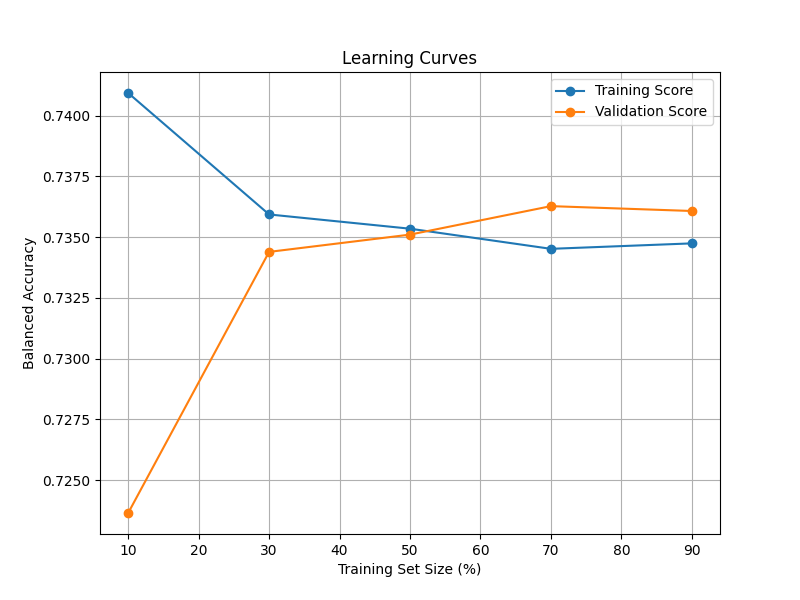
\includegraphics[width=0.95\columnwidth]{figures/learning_curves.png}
    \caption{Learning curves showing model improvement over training iterations.
    The solid lines represent training metrics while dashed lines show validation metrics.}
    \label{fig:learning}
\end{figure}

The progression of our model showed significant improvements:
\begin{itemize}
    \item Baseline model: All predictions negative (accuracy = 0.5)
    \item After class balancing: Improved detection of positive cases
    \item Final model: \textbf{Balanced accuracy of 0.717} (evaluated using AICrowd platform)
\end{itemize}

\subsection{Feature Analysis}
\begin{figure}[H]
    \centering
    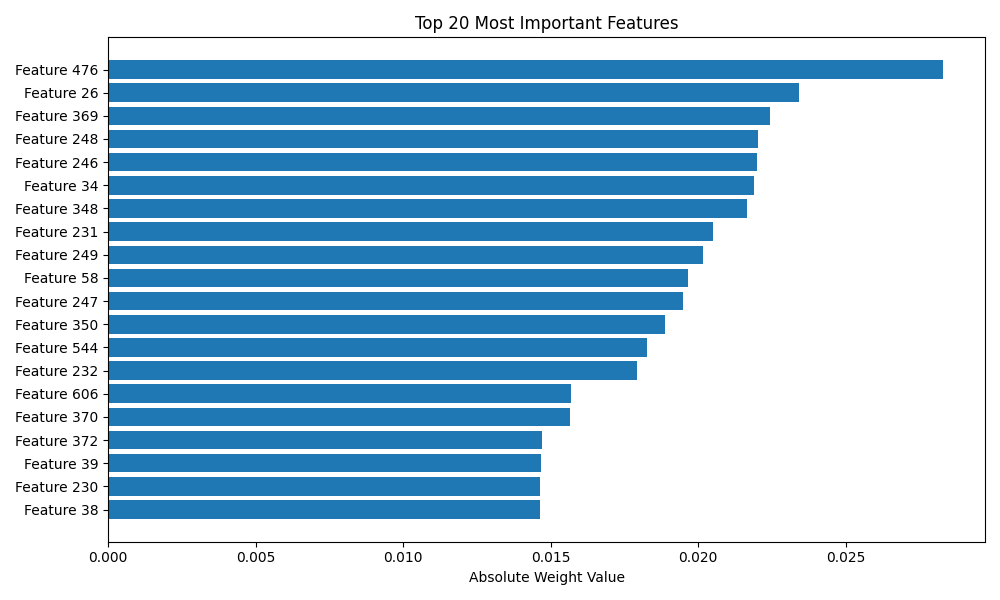
\includegraphics[width=0.95\columnwidth]{figures/feature_importance.png}
    \caption{Relative importance of health indicators in prediction. 
    Features are sorted by their absolute coefficient values in the logistic regression model.}
    \label{fig:features}
\end{figure}

\section{Implementation Details}
The complete implementation of this project, including data preprocessing pipelines,
model training scripts, and evaluation metrics, is available in our public repository:
\url{https://github.com/superflash41/epfl-ml-project-1}. The repository includes:

\begin{itemize}
    \item Documentation related to the project, including data sources and model details
    \item Python scripts for model training and evaluation
    \item Requirements file for environment reproduction
\end{itemize}

\section{Discussion}

The evolution from our initial implementation to the final model reveals several key
insights about medical data classification:

\begin{itemize}
    \item Class imbalance significantly impacts model performance in medical predictions
    \item Feature engineering and proper scaling are crucial for capturing health indicator
    relationships
    \item Adaptive learning rates help stabilize training with imbalanced data
\end{itemize}

Our final model achieved meaningful predictions for both classes, demonstrating the
effectiveness of our enhancements. However, there remain opportunities for improvement:

\begin{itemize}
    \item Investigation of more complex feature interactions
    \item Exploration of ensemble methods for robust predictions
    \item Integration of domain-specific medical knowledge in feature engineering
\end{itemize}

\section{Personal Context and Future Research Interests}

This project was developed individually as part of the CS-433 Machine Learning course from EPFL.
While I haven't formally taken AI or ML project-based courses at PUCP,
this work represents my self-driven interest in the field. Through this project,
I aimed to demonstrate not only my ability to implement and improve machine learning
algorithms but also my commitment to understanding their theoretical foundations.

My experience with this project has strengthened my interest in pursuing further studies in AI,
particularly in theoretical AI research. \textbf{I am especially intrigued by the concept of
compositionality in deep learning models - how these systems can learn to combine and reuse
basic components to solve complex tasks.} This interest aligns with my future academic goals,
including potential thesis work focusing on the theoretical aspects of AI systems.

The progression from a basic logistic regression implementation to handling real-world
challenges in this project has provided valuable insights into both practical
and theoretical aspects of machine learning.

\section{Summary}

We successfully developed a heart disease prediction model that overcomes the challenges of
imbalanced medical data. The progression from a naive implementation to a more sophisticated
solution demonstrates the importance of careful consideration of data characteristics in
medical applications.

\end{document}